\documentclass[a4paper]{article}

\usepackage[english]{babel}
\usepackage[utf8x]{inputenc}
\usepackage{amsmath}
\usepackage{graphicx}
\usepackage[colorinlistoftodos]{todonotes}
\usepackage{tikz}
\usetikzlibrary{trees}

\title{Machine Learning Homework \# 4}
\author{sakohl, milsen, jkirchner}

\begin{document}
\maketitle



%\section{Exercise}
\begin{figure}
\centering
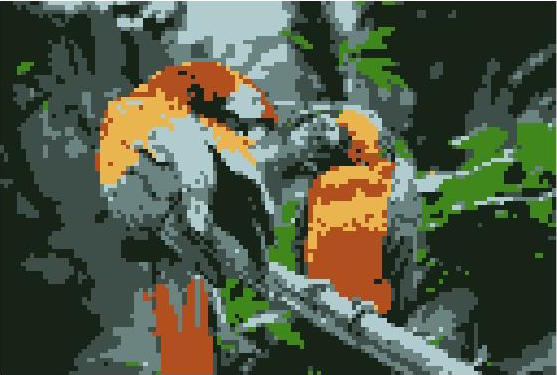
\includegraphics[width=0.3\textwidth]{8bitkmeans.jpg}
\caption{\label{fig:8bit}8 bit k-means}

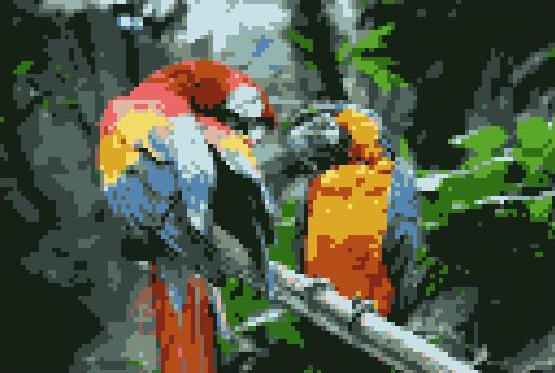
\includegraphics[width=0.3\textwidth]{16bitkmeans.jpg}
\caption{\label{fig:16bit}16 bit k-means}

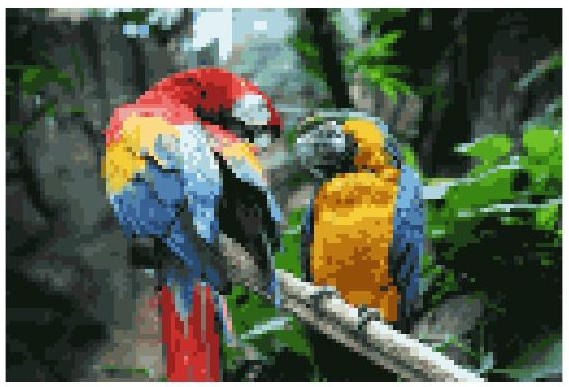
\includegraphics[width=0.3\textwidth]{64bitkmeans.jpg}
\caption{\label{fig:64bit}64 bit k-means}
\end{figure}

\end{document}